\chapter{Improvement of Visual Odometry}\label{Chap:Imp}
Above the procedure of self-localization was described in general. Both unscented Kalman filter and particle filter will require the pose information which provided by visual odometry part. So the accuracy of pose estimated by visual part will definitely have an obvious influence on the final result.
\clearpage
\section{The current method}
\subsection{Visual odometry procedure}
There are several sensors to acquire information from the environment on NAO: camera, microphone and sonar. From them only the camera is adopted, since the environment of the soccer match will be quite complicated, for example:
\begin{itemize}
    \item The white border lines and green field are on the same plane.
    \item The goal posts are perhaps too far away from the robots sometimes.
    \item There are 6 moving robots on the field, which the opponents are distinguished from our teammates only by colors.
    \item The ball is small and the detection of a ball requires high precision.
\end{itemize}
So based on above reasons, the another sensors are not qualified for the requirements. However, the camera is suitable for each specific task and the computer vision skill as well as visual odometry are being perfect so far.

There two cameras on the NAO's head shown in fig, which can provide large FOV. Several tasks such as image preprocessing, feature detection(including: line perception, penalty mark perception, ball perception) and data association will be performed on the image gathered by each camera. The features on the football field will be described as ``X" crossing, ``T" crossing and ``L" crossing which can be associated to the feature detected in pixel images. The detailed of these tasks will not be mentioned in my part of report, which are introduced by my teammates. My work is that suppose the the feature detection and data association have been finished.
Based on feature detection and data association, the corresponding point pairs have been already found. For example the goal post in figure i. whose coordinate in the homogeneous global 3D world could be represented as $(X,Y,0,1)^T$. And the corresponding homogeneous coordinate in pixel coordinate can be written as $(x,y,1)^T$. Since the camera callibration matrix, including both intrinsic and extrinsic calibration parameters, has been acquired through camera calibration %Bhumancoderelease
 before each match. Assuming the camera model as pinhole camera model: % put a calibration image
\[ % without number
x = K 
\begin{bmatrix}
a & b \\
c & d 
\end{bmatrix}
\]
%\begin{figure}[!htb]
%    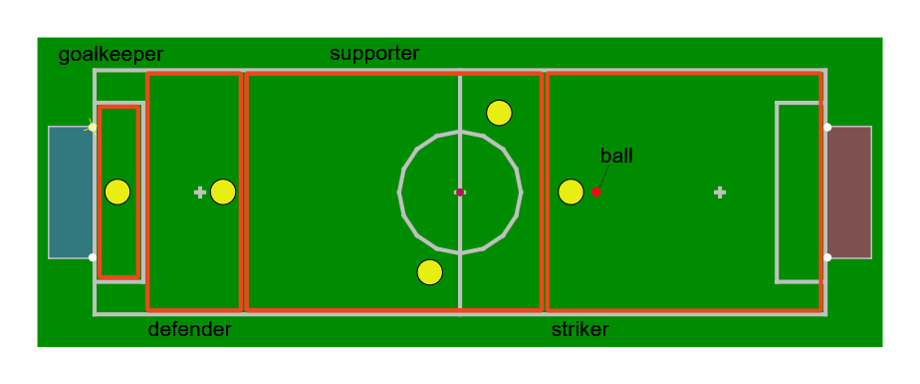
\includegraphics[width=0.9\textwidth]{pics/SPL}
%    \centering
%    \caption{Roles in SPL}
%    \label{fig: SPL}
%\end{figure}\\
%For the RoboCup at TUM, there are three robots in each team, namely the goal-keeper, defender and striker as shown in \fref{fig: TUM}. The original behavior of these roles are from B-Human CodeRelease in \cite{BHumanCodeRelease2015}.

So we could get the corresponding goal post coordinate in the ideal camera frame. Since we know the geometrical value of NAO's body construction, we can transform the coordinates into the robot frame, which is shown in the figure % coordinate transform
Based on this, we could get the related distance between robot and the goal post in robot frame. At the same time, the pricise location of goal post in the global field is also known. So we could calculate the robot pose from this above information. % show the calculation procedure

\subsection{Current problem}
In the process of transforming the coordinate from camera frame into robot frame, the current method only use a constant transform. However
